\documentclass[a4paper,oneside]{report}

\usepackage{amsmath}
\usepackage{amssymb}
\usepackage[english]{babel}
\usepackage{fancyhdr} 
\usepackage{multirow}
\usepackage[pdftex]{graphicx}
\usepackage{listings}      
\usepackage{pdfpages}
\usepackage{setspace}
\usepackage{url}

\makeatletter



%
% Some custom definitions
%

% add horizontal lines
\newcommand{\HRule}{\rule{\linewidth}{0.5mm}}
\newcommand{\HRuleLight}{\rule{\linewidth}{0.1mm}}

% custom part page
\def\part#1#2
{
	\par\break
  	\addcontentsline{toc}{part}{#1}
	\noindent
	\null	
	\HRuleLight\\[0.0cm]
	\vspace{20pt}	 
	\begin{flushright} 		
  	{\Huge \bfseries \noindent #1}\\
  	\vspace{30pt} 
	\begin{minipage}{0.85\textwidth}
		\begin{flushright}
		{\large \noindent #2}
		\end{flushright}
	\end{minipage}\\[0.75cm] 
	\end{flushright} 		
	\thispagestyle{empty}
	\break
}

% chapter header
\renewcommand{\@makechapterhead}[1]
{\vspace*{50\p@}{
	\parindent \z@ \raggedright \normalfont
	%\huge \bfseries \thechapter. #1
	\huge \bfseries #1
	\vspace{20pt}}}

\setcounter{secnumdepth}{-1} 
\onehalfspace
\oddsidemargin 1in 
\oddsidemargin 0.6in 
\topmargin -0.3in
\setlength{\textwidth}{14cm}
\setlength{\textheight}{23cm}
\lstset{language=C} 

\begin{document}

%
% Cover page
%
\begin{titlepage}
\begin{center}


\includegraphics[width=120mm]{sources/images/cogito_logo_main.png}

\HRuleLight\\[0.5cm]

\begin{minipage}{0.45\textwidth}
	\begin{flushleft}\large
		\emph{Author:}\\
			\textbf{Thomas \textsc{Taylor}}\\[0.27cm]
			Computer Science (Games)
			Student Number: 08813043
	\end{flushleft}
\end{minipage}
\begin{minipage}{0.43\textwidth}
	\begin{flushright} \large
		\emph{Supervisor:} \\
		\textbf{Graham \textsc{Winstanley}}\\[0.25cm]
		\emph{Second Reader:}\\
		\textbf{Saeed \textsc{Malekshahi}}
	\end{flushright}
\end{minipage}\\[0.75cm] 

\HRuleLight\\[0.2cm]

\large School of Computing, Engineering and Mathematics\\ \textbf{University of Brighton}

\vfill
\huge Project Documentation\\
\large April, 2012\\

\end{center}
\end{titlepage}



%
% Table of contents
%
{
	\renewcommand\thepage{}
	\setcounter{tocdepth}{1}
	\tableofcontents
	\clearpage
}

% reset page count
\setcounter{page}{1}


%
% Start of content
%

\chapter{Introduction}

The artificial intelligence (AI) techniques utilised by game developers have been called archaic by the academic AI researchers, which may indeed be true. However, it is important to view such techniques in context of which they are used. While academic AI researchers are able to utilise as much processing power as the hardware can afford them, game developers are much more limited. When one examines the other processes which need to run concurrently, this is not overly surprising: physics, sound, networking, input and most importantly the graphics processing to name but a few. So when AI researchers complain that the techniques are archaic, which is a fair arguement, given that the A* search algorithm is still one of the most popular AI algorithms used in games today, and was first introduced over 30 years ago), this is for the simple reason that the amount of processing power that developers are able to dedicate to the AI processes could not cope with any more `recent', processor intensive techniques. Indeed, modern game AI programming is more a skill of employing the cheapest (computationally) techniques, and often means that shortcuts and workarounds are a necessity in order to achieve `believable' AI. 

However, this being said, we are starting to see a change taking place in the computer games industry which suggests that the processing time availiable for often overlooked processes such as AI is starting to increase. One such factor in this change is the so-called `graphics plateau' \cite{Sheffield:2008fk}. Whether or not there will come a point where the graphical complexity of a game is considered `perfect', with no area for improvement is uncertain (and in my opinion highly unlikely). However, I do think that we have reached a point whereby the graphical complexity achievable with each new generation in games consoles is unlikely to achieve the same kind of drastic improvement in detail that we have seen over the last couple of decades; in effect, I think that we have reached a level of complexity whereby the amount of processing power needed for the graphics processing is unlikely to increase by a very large factor. Given the inevitable hardware advances that come with each new generation, I believe that we will start see a lot more processing power freed up for those processes which have been treated as `extraneous' in the past, such as the AI. 

Another important factor in this change is the emergence of the `casual' gamer. With casual games now accounting for a considerable proportion game sales, the consumer has shown that there is a big market for games which have less emphasis on complex graphics effects, and more emphasis on interesting gameplay mechanics \cite{Association:2011uq}. Indeed, with Nintendo's Wii home console having far outsold both Sony's PlayStation 3 and Microsoft's Xbox, the consumer has shown that they value unique gameplay and accessibility over advanced graphics \cite{:2012dq, Nintendo:2012nx, :cr}. 

\paragraph{USER BASE PIE CHART}\ \\ \\

With these factors already starting to bring about a change in the priority that developers give to the components of their games, I believe that now is as good a time as any for developers to introduce some more advanced AI techniques into their games.

\section{Project Aims and Objectives}

My main aim with my project was to experiment with some more advanced academic AI techniques which are not typically found in commercial games today for various reasons, and look into whether such techniques were actually viable with today's hardware. This second point is key, especially given the popularity of fairly limited hardware such as the Nintendo Wii, and mobile hardware.

The sub-field of AI that I chose to focus my project on was machine learning, as it is an emerging field which greatly interests me and one which I feel is a natural fit for computer games, and one we could see utilised in many forms in future games.

For my project, I wanted to develop an AI system which was capable of employing machine learning techniques in order for a number of AI-controlled agents to safely navigate a 2D game environment. I wanted the agents to be able to develop a knowledgebase dynamically, with no need for prior training, or knowledge of the game world. I then wanted the agents to be able to apply this gained knowledge in order to hopefully increase their chances of survival. 

\section{Background}

I chose the classic Commodore Amiga game `Lemmings' as the context and main inspiration for my project.

\begin{figure}[h!]
  \centering
    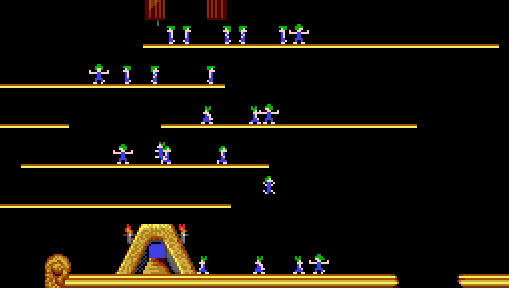
\includegraphics[width=100mm]{sources/images/lemmings3}
    \caption{A typical level in Lemmings.\label{screen}}
\end{figure}

Originally released in 1991 for the PC and Commodore Amiga, `Lemmings' has a very simple premise: to guide a group of computer-controlled `lemmings’ across a level from the entrance-point to the exit. The Lemming characters themselves have very basic AI; capable of merely walking across the level map. The level itself consists of a number of platforms, along with a number of hazards which will kill the Lemmings (big drops, pits etc.). The goal of the player is to utilise a set of tools in order to ensure that the Lemmings safely reach the level exit, such as umbrellas for big drops, girders to cross pits etc. 

For my project, I planned to take this concept, simplify it by removing some of the tools and obstacles, and program some AI agents to learn for themselves how to best traverse the level, without any human interation.
		
\section{The Project in Context}
	
Throughout the development of my project, I needed to utilise skills which I had gained from modules I had studied during my course.

There was obviously a lot of knowledge that I gained in the AI-related modules I have studied (CI213 - Intelligent Systems and CI342 - Advanced AI) which I could directly apply to my project. Techniques such as pathfinding algorithms, and generally approaching AI-based problems from an academic angle.

I was also able to apply a lot of useful knowledge that I had gained from the programming-based modules from my course (CI101 - Introduction to Programming, CI228 - Object-Oriented Software Design and Specification and CI346 - Programming, Concurrency and Client-Server Computing). I applied a lot of the `good' object-oriented design practices which were learnt in these modules: principles such as inheritance and design patterns like the singleton. I also found the knowledge learnt this year in CI346 very useful to overcome some concurrency issues I had using multiple threads in my system.

Another module I have found to be very useful is CI224 (Games Development). Many of the game design concepts: physics, object transformations, model loading, and various other useful skills. The project we did in CI224 was particularly useful, as it introduced me to the process involved in developing a game from scratch. I was also introduced to source control systems in CI224, which has proven to be invaluable knowledge to have.

I also used the knowledge of object-oriented software design and UML learnt in CI228 and CI231 (Formal Underpinnings and Specification) to design my system. Although I didn't actually use the formal specification language learnt in my system specification, I could still apply the concepts learnt to my own designs.

I learnt a great deal about data access and performance optimisation in the CI312 (Computer Graphics Algorithms) module. It really helped me too look at my code at a lower level, and analyse the best and most efficient ways to access and manipulate data; something which I have found to be incredibly important, especially in a game context, where some functions can be called 60 times every second. This is something which is of paramount importance, especially in games, as you will likely be carrying out certain functions up to 60 times every second, so any inefficient code would cause big problems in performance. 



%
% New part
%

\part{Research}{This section documents the research that I carried out prior to designing my system, and how it influenced my final designs. \\ \ \\The section is split into two subsections: my research into AI, and my research into the more game-related topics.}

\chapter{Artificial Intelligence}

Since the early days of `modern' computing, computer scientists have striven to replicate in machines the defining characteristic that makes us human: intelligence. One of the first references to `intelligent machines' came in 1950 in Alan Turing's seminal paper \emph{Computing Machinery and Intelligence}, in which Turing opens with the words: "I propose to consider the question, 'Can machines think?'". In it, he outlines a test in which a human participant engages in conversation with a machine designed to imitate human behaviour, known as the Turing Test. This paper not only inspired the concept of `intelligent machines', but also caused us to look philosophically at what it is that makes us inherently human, and whether this is indeed replicable in a machine.

The term `artificial intelligence' was later formally defined in 1955 by McCarthy et al in the proposal for the Dartmouth Summer Research Conference on Artificial Intelligence, which is considered by many to be the origin of the field of AI \cite{Crevier:1993kl}. In the proposal, it was suggested that ``every aspect of learning or any other feature of intelligence can in principle be so precisely described that a machine can be made to simulate it" \cite{McCarthy:1955ve}. However, despite this early optimism, we are still yet to see any truly `intelligent' machines nearly 60 years on. Indeed, the annual Loebner Prize event in which AI researchers partake in Turing Tests has yet to award the silver or gold medals to any entrant. 

Since these very early days, the field of AI has grown to become an integral field not only in computer science, but also in the infrastructure of every industry \cite{Kurzweil:2005ly}. AI techniques are used in a vast array of application areas, such as in search, elevator scheduling, satellite monitoring, weather prediction, aeroplane autopiloting and robotics to name just a very few. 

\section{AI In Games}

One area where AI techniques are used extensively is computer games. Whether to map a route across obstacle-ridden terrain, control the actions of non-player characters (NPCs) or even to adjust game parameters to fit to the skill of the player, AI plays a key role in almost all modern computer games. 

However, despite the proven benefits of AI, the amount of system resources allocated to AI processing is surprisingly limited; traditionally, the game industry has been much more focussed on producing ultra-realistic visuals than with developing a truly intelligent AI system. With each new console generation, developers have pushed the hardware to its limits, offering greater levels of visual fidelity while other areas of development were neglected. It is no surprise then, that game AI programmers have had to make the best of a bad situation, often being forced to avoid  more powerful and resource-intensive AI techniques for a mixture of highly optimised (and less-effective) techniques, and a `smoke and mirrors' approach.

Due to the nature of the final product, game AI takes a very contrasting approach to that of academic AI. While the aim with academic AI systems is always to provide the most complete and accurate results, the ultimate aim with game AI is to provide entertainment for the user, by giving the illusion of intelligence. Ironically, this can often mean that it is necessary to make the system intentionally `stupid' by building flaws in the system or even by allowing the system to cheat to ensure that the game AI behaves `realistically' \cite{Liden:2004fk}. Additionally, academic AI systems usually have the very simplistic interfaces or visualisation, in order to allow the majority of processing time to be dedicated to the AI. In a computer game on the other hand, the AI must run simultaneously with a number of other processes such as the physics engine, sound and most importantly graphics which in reality means that the AI processing is often compromised in the favour of other processes.

The AI systems used in most modern games mainly concern themselves with the following three objectives \cite{millington2006artificial}:

\begin{itemize}
	\item The ability to move characters
	\item The ability to make decisions about where to move
	\item The ability to think tactically or strategically
\end{itemize}

In the proceeding sections, I outline some of the most popular AI techniques used in commercial computer games today.

\subsection{Finite State Machines} 

Finite state machines (FSMs) are one of the most basic and most commonly used AI techniques found in games today. As the name suggests, finite state machines are ``simple, rule-based systems in which a finite number of 'states' are connected in a directed graph by 'transitions' between states" \cite{:hc}. This graph essentially maps the states available, and which of these states can be reached from the current state. One of the first games to sucessfully implement FSMs is Atari's 1979 game \emph{Pacman}, in which the enemy ghost characters use a FSM to either roam around, chase Pacman or run away, changing their state in response to various in-game triggers. Despite the age of this technique, it is still used extensively in many commercial games today, due to the fact that FSMs are fairly easy to understand, easily implementable, and most importantly, relatively straightforward to debug \cite{Bourg:2004tg}.

\subsection{Search and Planning Systems} 

Search and planning systems have many different uses and are used extensively in many different genres of games. Search systems are primarily concerned with finding actions or states in a graph in order to satisfy a goal condition (or at least to get as close as possible to the goal condition). Planning systems are a branch of the search methods which have an emphasis on finding the best (or simplest) sequence of actions required in order to reach a goal state. There have been a variety of search algorithms developed over the years, but the A* algorithm is the one used most extensively, due to its performance, and the accuracy of its results. Search and planning systems are used for a variety of tasks, from the pathfinding of AI agents in a first-person shooter game to the allocation of resources in a real-time strategy game. Blizzard's 1994 game \emph{Warcraft} is an example of an early implementation of using the A* pathfinding algorithm to navigate agents.

\subsection{Artificial Life} 

The use of artificial life (A-life) techniques have become more commonplace in recent years, and have a variety of different uses. An A-life system is essentially system which is designed to exhibit realistic and lifelike behavior in game characters. A-life systems are often used to coordinate the movement of multi-agent systems to make the agents maneuver in flock and herd formation. One of the most compelling reasons to use A-life techniques is that more complex intelligent behaviours can emerge as a result from the pre-programmed rules \cite{Woodcock:bs}. \emph{The Sims} developed by Maxis (now part of EA) is probably one of the best known games to use A-life techniques, and uses so-called `smart terrain' to broadcast information to the game characters. For example,  a character which is hungry may walk past a refridgerator, which broadcasts that it contains food. After collecting the food, the nearby oven may broadcast that it can cook the food, leading the character to it \cite{Woodcock:bs}. These individual object-level actions when combined, cause the character to act realistically. While A-life techniques can result in some very realistic and emergent behaviour without having being explicitly programmed to do so, it also means that the unpredictability which is inherent to A-life can mean that it can be incredibly difficult to debug. Additionally, the more complex techniques can be incredibly processor intensive, rendering them unsuitable for games which are already very processor-intensive. 

\subsection{Scripting} 

Another popular technique in game AI is scripting, whereby developers use a specialised high-level scripting language to outline the NPCs reactions to basic situations as well as to hard-code game events. Scripting allows the game engine to be accessed externally in a safe `sandbox' environment, greatly reducing the chance of bugs and errors, so is suitable for non-programmers such as designers, or even end-users to access. For this reason, there is a large community of gamers which build additional content for various games via the scripting interface. Common uses for scripting include creating events and controlling the enemy AI. 

Lionhead used scripting heavily in their 2001 game \emph{Black \& White} to present the game's storyline using a series of in-game challenges rather than the more traditional cut-scene, as well as to implement the game's logic \cite{:hc}. 

A big disadvantage to using scripting is that it requires every character behaviour and game scenario to be hard-coded which is incredibly time consuming for the programmer/developer, and is not always possible. Additionally, using scripting can be very restrictive for the player, as the story progression is often very linear.

\subsection{Cheating The System}

In addition to the AI techniques outlined above, many developers also use a number of hacks and workarounds to give their AI systems the illusion of intelligence while retaining the entertainment value. In many cases, the more traditional AI techniques aren't needed at all. As discussed earlier, the primary aim when it comes to game AI is to make the AI system appear `intelligent' whilst at the same time presenting an acceptable level of challenge for the player. If we examine a stealth action game such as Konami's \emph{Metal Gear Solid} series in which the player must traverse a level while avoiding detection from the guard NPCs; were a truly intelligent and adaptive AI system used which was able to reason as completely as the player, it would remove a lot of the entertainment value of the game which often relies on the player recognising patterns in guard behaviour in order to progress. While this AI system would be considered flawed in the eyes of an academic researcher, it is perfectly acceptable in the context of the game. Similarly, game developers often give the AI system access to extra information or resources which are unavailable to the player. This is particularly the case with real-time strategy games (RTSs) where it is commonplace for the enemy player to have access to extra resources such as troops or supplies which wouldn't be available to the player. Using these kinds of `cheats' can be an acceptable way to increase the level of difficulty. However, the challenge for the developer is to disguise this from the player; if the player feels that the game is acting unfairly, and that their actions are ineffective, they will obviously not enjoy the game.

\subsection{The Future of Game AI}

From as early as 2000, statistics were showing that the industry was beginning to take AI more seriously. This was reflected in figures collected from the AI roundtable at the annual Game Developer's Conference (GDC), which showed that not only were a lot more studios employing dedicated AI programmers, but also the average amount of CPU time reserved for AI processing increased from 5\% to over 25\% \cite{Woodcock:oq}. With increased resources now available to AI developers, there is more opportunity now than ever to introduce newer and more advanced AI techniques such as neural networks and machine learning.

\section{Machine Learning}

\begin{quotation}``A computer is said to learn from experience \emph{E} with respect to some class of tasks \emph{T} and performance measure \emph{P}, if its performance at tasks in \emph{T}, as measured by \emph{P}, improves with experience \emph{E}." - \textbf{Tom Mitchell} \cite{mitchell1997machine} 
\end{quotation}

The ability to learn is one of the central features of intelligence \cite{Langley:1996zr}. To be able to then apply this knowledge and modify behaviour accordingly when faced with similar scenarios in the future is an area which has recieved a considerable amount of research, with techniques having been developed to tackle a wide variety of learning problems. In fact, machine learning techniques are already in use in a number of commercial applications such as speech recognition, robotic control and machine vision, proving that it can be a very useful solution, especially in solving problems which may have unexpected outcomes that cannot be predicted by the software developer.

\paragraph{} Learning techniques can be classified into various groups based on what is learnt, when learning occurs and the effects that the learning has on the system. 

\paragraph{Online and Offline:} Learning which takes place while a system is running is said to be `online', while `offline' learning refers to a system which modifies its behaviour \emph{after} it has finished running. Whilst online learning provides instantaneous results, it also makes the system much more difficult to debug were any issues found, due to its continous modification.

\paragraph{Supervised and Unsupervised:} Learning which utilises example training data is described as `supervised', whereas a system which only has access to the data that it collects itself is described as `unsupervised'. The benefit to supervised learning is that the system can base its learning on some correct `solutions', which lead to more accurate and perhaps `quicker' learning. However, the training data itself needs to be collected and analysed, which requires human input, and can become very time consuming. Unsupervised methods on the other hand do not have this requirement, but must analyse the collected data to find hidden structure; there is no `correctness' indicator to evaluate potential solutions. There are also techniques which form an intermediary between the two, using both labelled and unlabelled data. These methods are known as `semi-supervised'.

\subsection{Reinforcement Learning}

Reinforcement learning (RL) is the name given to the subset of machine learning techniques which use a reward signal system to let the system know how it is performing; the overall aim being to maximise the cumulative reward. Originally inspired by animal behaviour, RL is centred around one of the fundamental ideas underlying many theories of learning and intelligence: that we learn by interacting with our environment \cite{Sutton:2005kl}. 

RL uses a cause and effect loop whereby the system begins in a state, performs an action (recieving a reward). causing the environment change its state, and repeating the cycle (see Figure 2).

\begin{figure}[h!]
  \centering
    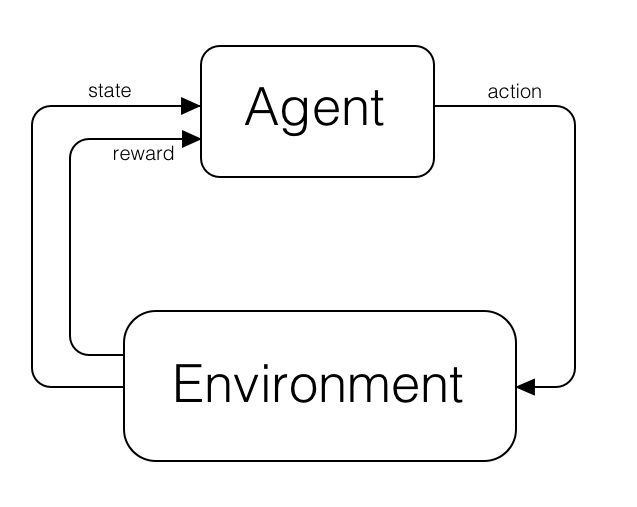
\includegraphics[width=70mm]{sources/images/RLDiagram}
    \caption{The Reinforcement Learning Loop \cite{Nilsson:2010qa}.\label{screen}}
\end{figure}

What sets RL apart from other types of machine learning (i.e. supervised/unsupervised methods) is that the learner is never given correct input/output pairs, nor are any incorrect (or sub-optimal) actions ever corrected, leaving the system to deduce where an error has occurred for itself. This can be particularly tricky to ascertain as an error can often occur due to a poor decision made several timesteps in the past. Similarly, the mistake could have been made as a result of 20 previous actions, all of which would have to be repeated in sequence to replicate the error. This is known as the `credit assignment problem', and results from the fact that RL uses a sequential style of learning, where a system makes many decisions which lead to an eventual goal condition. In an attempt to combat this, RL introduces the notion of `regret', by taking into account the long-term effects of its actions. For example, an RL system may choose an action with a negative immediate reward so as to maximise its long-term reward.  

RL also has an emphasis on performance, which involves finding an acceptable compromise between exploration (of new undiscovered terrain) and exploitation (of the system's current knowledgebase).

\subsubsection{Markov Decision Processes:}

When designing an RL system, it is necessary to represent the environment in which the system is intended to be used. A mathematical structure known as a Markov Decision Process (MDP) is often used for this purpose. An MDP is usually represented as follows:

\begin{equation*}
MDP(S, A, \{Psa\}, \gamma, R)
\end{equation*}

\noindent and consists of 5 main components: 

\begin{enumerate}
	\item A set of possible states \emph{S}
	\item A set of available actions \emph{A}
	\item State transition distributions \emph{Psa}, which gives you the probability \emph{P} of transitioning to a new state \emph{$s^\prime$} if you take some action \emph{a} while in state {s} (value can be 1)
	\item The discount factor $\gamma$ where 0 $\leq \gamma \leq$ 1 (a value chosen by the programmer which adjusts how much influence future rewards have)
	\item A reward function \emph{R}, which can be positive or negative, and maps from a state to a real number $R : S \mapsto \mathbb{R}$ (also an arbitrary value chosen by the programmer)
\end{enumerate}

MDPs are very useful when implementing RL systems in particular as they encapsulate all of the required information: which actions are available in the current state, which states the system can can transition to next, the probability that the system will transition to the next state, and the reward for reaching the state.

\subsubsection{The Theory} 

In order for the algorithms to compute an optimum policy, the system must first build up a knowledgebase through experience. It does this simply be executing:

\paragraph{} Starting in some state $s_0$ and performs some arbitrary action $a_0$ (often chosen at random during this learning phase), causing the system to transition to the next state $s_1$ according to the probability function for the current state and action $Ps_0a_0$. The probability function is not always necessary, but there may be circumstances where it does apply. As an example, you may have a robot with an inaccurate direction sensor, which when set to move north, causes it to move in the desired direction 80\% of the time, with a 10\% of going east, and a 10\% chance of going west.

\paragraph{} After running for an arbitrary amount of time, the system will have reached a number of different states: $s_0, s_1, s_2, s_3 ...$ We can now evaluate the performance of the system using some reward function, whereby the cumulative rewards would be:

\begin{equation*} 
	R(s_0) + R(s_1) + R(s_2) + R(s_3) + ...
\end{equation*}

\paragraph{} The final step is to incorporate the discount factor into the calculation. Incorporating the discount factor into our equation gives us the following: 

\begin{equation*} 
	R(s_0) + \gamma R(s_1) + \gamma^2 R(s_2) + \gamma^3 R(s_3) + ...
\end{equation*}

Whereby the reward received at timestep $t$ is discounted by $\gamma^t$. This approach gives a greater weighting to rewards now than to rewards in the future.

\paragraph{} The ultimate goal of the RL algorithm is to formulate a policy\footnote{The term `policy' is used to refer to a set of action/state mappings often symbolised by $\pi$} which maps the states to the actions ($\pi: S \mapsto A$) such that for every state, the policy recommends the optimum action to take.

\paragraph{} After a certain number of iterations of the RL algorithm, the policy would reach a point where its values become static (i.e. they are no longer updated with each iteration). This signifies that the optimum policy has been found, and the values have \emph{converged}. For very small problems, this could take a few thousand iterations, but is likely to take a vast amount more for complex problems. In many real-world cases, there may not be enough time to feasibly reach convergence, in which case the best policy would be used.

\paragraph{} Although each RL algorithm varies in its implementation, these are the basic concepts which underly all methods. 

\subsubsection{Algorithms}

There have been a variety of different RL algorithms developed, each with their own advantages and disadvantages. I outline some of the most popular algorithms in this section. 

\subsubsection{Policy Iteration}

\subsubsection{Dynamic Programming} 

One approach to RL is dynamic programming, a method most commonly used in solving learning problems in which the state transition probabilities are known beforehand.

The state transition probability function, $p(s,a,s^\prime)$ is the probability of transitioning from state $s$ to state $s^\prime$ when the agent takes action $a$. The goal of the learning agent is to learn to approximate the reward function $V(s,a)$, which gives the expected reward of taking action $a$ in state $s$. The agent approximates the reward function by testing out different actions in different states, each time receiving a reward $r$. For taking action $a$ in state $s$, the agent updates $V(s,a)$ with the following function:

\begin{equation*}
V(s,a) \Leftarrow r + \gamma * \sum(p(s, a, s_\prime) * V(s_\prime))
\end{equation*}

Where gamma is a parameter known as the discount rate, the summation sums over all states s` and V(s`) represents the maximum V(s`,a) for all actions a. This equation is known as the Bellman equation.

\subsubsection{Temporal Difference} 

Temporal Difference methods are used to solve problems where $p(s,a,s_\prime)$ is not known. Temporal Difference solves the learning equation by using the expected reward of the next state it encounters after taking an action a in state s. The full equation is:

\begin{equation*}
V(s,a) \Leftarrow V(s,a) + \alpha * ( r + \gamma * V(s_\prime) - V(s,a) )
\end{equation*}

Where alpha is a parameter known as the learning rate. 

\subsubsection{Monte Carlo} 

Monte Carlo is similar to Temporal Difference but keeps track of all rewards encountered until an episode terminates in addition to the one state look-ahead performed by temporal difference methods.

\subsubsection{Bucket Brigade}

\subsubsection{Q-learning}

Another popular RL algorithm is Q-learning. Originally proposed by Christopher Watkins in 1989 \cite{Watkins:1989mi}, the Q-learning algorithm takes a slightly different approach to other RL algorithms, as it doesn't require a complete model of the environment, which can be a big advantage in certain scenarios, as it is not often not possible (or indeed feasible) to generate a model before the system has run.

Q-learning gets its name from the quality information, or Q-values which it stores for each state and action in the environment. For each possible state-action pair, the system stores a unique Q-value which represents how good it thinks that action is to take when in that state .

``The Q-value represents how good it thinks that action is to take when in that state."

\noindent The Q-learning algorithm is as follows:
\begin{equation*}
	Q(s_t,a_t) \Leftarrow Q(s_t, a_t) + \alpha_t(s_t, a_t)[R(s_t) + \gamma max_{a_{t+1}} Q(s_{t+1}, a_{t+1}) - Q(s_t, a_t)]
\end{equation*}

\noindent But is often rewritten more simply as:
\begin{equation*}
	Q(s_t,a_t) \Leftarrow Q(s_t, a_t) + (1 -\alpha_t) + \alpha[R(s_t) + \gamma max Q(s_{t+1}, a_{t+1})]
\end{equation*}

Where $Q(s_t, a_t)$ represents the Q-value for the current state/action, $R(s_t)$ represents the reward associated with the current state, $max Q(s_{t+1}, a_{t+1})$ represents the maximum possible Q-value for the next state

Updating the old Q-values ensures that the system retains all previously obtained knowledge. Introducing the max Q-value into the equation means that the success (or failure) of an action is reflected in earlier actions, in effect `trickling' back up the supply chain.

Q-learning converges with probability 1, meaning that after sufficient iterations of the algorithm, the learner can move towards the most desirable state from any location with little to no search .

``Thus, after sufficient experience, the problem solver can move toward the most desirable state from any location with little to no search"

\subsection{Decision Tree}

Another popular type of machine learning is Decision Tree Learning. Decision Tree Learning is 

Pros:
\begin{itemize}
	\item Relatively easy to use and understand; decision trees are easy to visualise and read
	\item Tree structures are a very commonly used data structure in computer science, and highly optimised algorithms for the building and searching of trees have already been developed
\end{itemize}

\noindent Cons:
\begin{itemize}
	\item Can lack accuracy; the size of the tree will increase tremendously to provide a higher resolution output \cite{schwab2004ai}.
	\item Trees don't scale well, and highly complex trees can be very difficult to maintain
\end{itemize}

Moreover, because agents need to learn online as the game is played, predetermined training targets are usually not available, ruling out supervised techniques such as backpropagation (Rumelhart et al. 1986) and decision tree learning (Utgoff 1989).

\subsection{Genetic Algorithms}

Pros:
\begin{itemize}
	\item When it may be too computationally expensive to calcuate a decision
	\item To complement other AI techniques
	\item Relatively simple to set up and start getting results, even if you don't know how to solve the problem otherwise
\end{itemize}

\noindent Cons:
\begin{itemize}
	\item Evolution is often time-consuming, taking many generations
	\item Not guaranteed to find an optimal or even satisfactory solution
	\item Don't cope well with components which may not have a concrete design; the addition of features can require a complete redesign of the genetic algorithm
\end{itemize}

\subsection{Artificial Neural networks}

attempt to model a brain

An artificial Neural Network (NN) is an electronic simulation based on a simplified human brain. In an NN, knowledge is acquired from the environment through a learning process and the network’s connection strengths are used to store the acquired knowledge [20].

Choosing the variables from the game environment that will be used as inputs is the most labour intensive part of developing an NN [30]. This difficulty is due to the fact that there is wealth of information that can be extracted from the game world and choosing a good combination of relevant variables can be difficult. Also, the number inputs needs to be kept to a minimum to prevent the search space from becoming too large [9]. Therefore, it is a good idea to start with the essential variables and add more if required. Choosing inputs that are poor representations of the game environment is the primary reason for failed applications.
NNs are techniques that can be used in a wide variety of applications. Some common uses include memory, pattern recognition, learning and prediction. There are many commercial applications of NNs across various industries, including business, food, financial, medical and health care, science and engineering [24]. Prominent companies that are using NNs include Microsoft, Sharp Corporation, Mars, Intel, John Deere, Mastercard, Fujitsu and Siemens [24]. Some examples of applications that NNs are being used for are predicting sales, handwritten character recognition for PDAs and faxes, odour analysis via electronic nose, stock market forecasting, credit card fraud detection, Pap smear diagnosis, protein analysis for drug development and weather forecasting. This list illustrates the wide variety of applications that can make successful use of NNs, and how their usefulness is only limited to what can be imagined.
The computer game industry is no different from the industries mentioned above in terms of the variety of applications of NNs. A few applications are described by LaMothe [26], including environmental scanning and classification, memory and behavioural control. The first application, environmental scanning and classification, involves teaching the NN how to interpret various visual and auditory information from the environment, and to possibly choose a response. The second application, memory, involves allowing the AI to learn a set of responses through experience and then respond with the best approximation in a new situation. Finally, behavioural control relates to the output of the NN controlling the actions of the AI, with the inputs being various game engine variables. Also, the NN can be taught to imitate the human player of the game [31].

Basically, an NN can be used to make decisions or interpret data based on previous input and output it has been given. The input can be seen as various games states, similar to that used by a state machine, and the output could be the action to be performed. The important difference is that the current state doesn’t need to have been hard-coded. Instead, the NN makes the best approximation that it can, based on the states that it already knows about. This means that the NN will choose an action that would have been performed in a similar state.

So far, game developers have been reluctant to allow a game to ship with the learning in NNs and other techniques “switched on”, in case the AI were to learn something stupid [46]. Therefore, the developers that have used NNs in their games have not used them for learning, but rather trained them during development and locked the settings before shipping. Some examples of games that include NNs for various tasks include BattleCruiser: 3000AD, Black \& White, Creatures, Dirt Track Racing and Heavy Gear.
In BattleCruiser: 3000AD (BC3K) the AI uses NNs to control the non-player characters as well as to guide negotiations, trading and combat [45]. It uses the development language AILOG (Artificial Intelligence \& Logistics), which was created by the developer of BC3K, Derek Smart, and uses an NN for very basic goal oriented decision making and route finding, with a combination of supervised and unsupervised learning. In Black \& White the player has a creature that learns from the player and other creatures. The creature’s mind includes a combination of symbolic and connectionist representations, with their desires being represented as NNs [15]. Finally, the Creatures series of games makes heavy use of Artificial Life techniques, including heterogeneous NNs, in which the neurons are divided into lobes that have individual sets of parameters. In combination with genetic algorithms, the creatures use the NN to learn behaviour and preferences over time.
In short, NNs are techniques that can be used for a wide range of applications in many different environments. Several commercial games have used this technique successfully, with the most recent and prominent being the game Black \& White. This technique’s flexibility means that it has the potential to be applied in a wide range of situations in future games. Therefore, it is likely that NNs will play a bigger role in commercial games in the near future.

\subsection{Applications For Machine Learning}

While it has yet to be utilised prominently in the game industry, machine learning is already used very effectively in many other application areas.

Tom Mitchell outlines many current application areas for machine learning in his 2006 article \emph{The Discipline of Machine Learning} \cite{Mitchell:2006fv}:

\paragraph{Speech recognition:} The commercial systems currently available all use some form of machine learning to train the system. Many systems even use a two-phase learning method: an initial phase for more general learning which is carried out prior to the product being shipped, and a second phase which tunes the system to the customer, and takes place after a customer purchases the product.

\paragraph{Computer vision:} Many of the currently available vision systems utilise machine learning techniques. One of the largest scale vision systems is in use by the US postal service to sort letters with hand-written addresses. According to Mitchell's paper, over 85\% of handwritten mail in the US is now sorted automatically using this system.

\paragraph{Robot control:} A further application for machine learning methods is for robotic control. For example, researchers at Stanford University lead by Andrew Ng have demonstrated a machine learning system capable of advanced helicopter flight \cite{Ng:2004dz, Abbeel07anapplication, Abbeel:fu}. This type of system could be particularly useful in space and planetary exploration in the future.

\paragraph{Accelerating empirical sciences} Machine learning methods are also being employed to aid in scientific discovery, such as gene analysis, in the field of astronomy for sky surveillance and to analyse brain activity. Machine learning methods are particularly useful in data-intensive areas for obvious reasons.

\subsection{Machine Learning In Games}

As discussed, machine learning techniques have been integrated into many different areas of computer science and indeed many other areas. However, such techniques have yet to reach the same kind of penetration in the computer game industry.

That being said, there has been a fair amount of research conducted by the academic community into the appliation of machine learning algorithms into a computer game environment. Additionally, there are already a few examples of commercial games which utilise such techniques to tremendous effect. 

\subsubsection{Academic Examples}

Machine learning techniques were first applied to board games such as checkers \cite{Samuel:1959qo, Samuel:1967ye}. In 2002, researchers David Fogel and Kumar Chellapilla created an evolutionary algorithm using neural networks to develop a checkers-playing system capable of beating its creators after just 10 generations \cite{Fogel:2003fk}. After 840 generations, the system was tested online on a competitive checkers website, where it reached the expert rating after 165 games, placing it in the top 500 of the 120,000 players on the site. While this is impressive, most board games emphasise only emphasise a few human capabilities such as search and decision-making \cite{Laird:2001tw}. 

In 2005, researchers at the University of Texas developed a reinforcement learning system known as rtNEAT which is capable of learning in real-time using neural networks and neuroevolution \cite{Stanley:2005ff}. Rather than simply playing games, the system is trained directly by the player in a `training mode'. In this mode, the player sets up training exercises by placing various objects and obstacles into the game world. The player can also adjust the algorithm's coefficients for fitness components using a number of slider interface elements. This allows the player to determine what they consider `ideal' behaviour, by adjusting how the AI characters disperse, use cover or approach enemies for example. I found this technique to be particularly interesting as it approaches the learning from a different angle, allowing the player to train the system themelves. Giving this kind of control and customisability over the AI's learning could be an attractive feature to players. 

In another example, researchers at the university of Maastricht conducted research as well as a number of experiments into a reinforcement learning-based technique known as `dynamic scripting' which uses ``an adaptive rule-base for the generation of game AI on the fly" \cite{Spronck:2005fu}. The experiments showed that after just 25 games, the dynamically scripted AI was able to develop a strategy to outperform the static AI for at least 10 consecutive encounters. This technique could be an attractive alternative to other machine learning techniques as it allows dynamic adaptive behaviours, while still allowing the developers to script certain behaviours, allowing more control than is typically possible with other methods.

A research group led by Robin Baumgarten developed an approach for ``simulating human game-play" using a variety of techniques built upon Introversion Software's 2006 strategy game \emph{DEFCON} \cite{Baumgarten:2008il}. The system displays an impressive level of intelligence through its planning of fleet movements and attacks as well as more low-level such as coordinating bombing runs and assigning bombing targets. To do this, the system maintains a knowledgebase of past games, which it uses to generate a plan for the current situation using a decision tree-based method. The system proved effective, with the system beating the static AI system in 76.7\% of games (of the 150 matches played). Most interesting about the research is the survey they conducted (albeit with a group size of 10 which is too small to be statistically significant). The results of the survey showed that the more advanced AI system was less popular with novice players, who felt a greater level of frustration and therefore less desire to play the game again. This is a very interesting point, as it demonstrates that game AI treads a very fine line between `fun' and `frustration'; while it may seem important to an academic researcher to develop a very strong adaptive AI system, the player would not necessarily show the same kind of enthusiasm.

\subsubsection{Commercial Examples}

Despite the promising academic research over the last decade, few developers have included machine learning techniques in their games. One of the few commercial games to employ such techniques to real effect was Lionhead Studios' god game \emph{Black \& White} \cite{:hc}. In \emph{Black \& White}, the player becomes a deity tasked with watching over a group of followers. Over the course of the game, the player must recruit as many followers as possible in order to gain influence over the land. To aid with this task, the player is given an AI controlled `creature', which the player must train to do his bidding. Lionhead implemented this learning using a combination of machine learning techniques; an approach they call `representational promiscuity', which is based on the idea that no single method could be used to build a complete agent. The creatures use a `Belief-Desire-Opinion-Intention' architecture to represent the creature's knowledge about the environment. When the creature percieves information in its environment, it is stored in memory as a `belief'. The creature uses these beliefs to form opinions which alter their desires in-game to suit the player. To form opinions about its environment, the creature builds decision trees by looking at attributes that best categorise the knowledge into groups (see Figure 3 for an example).

\begin{figure}[h!]
	\centering
		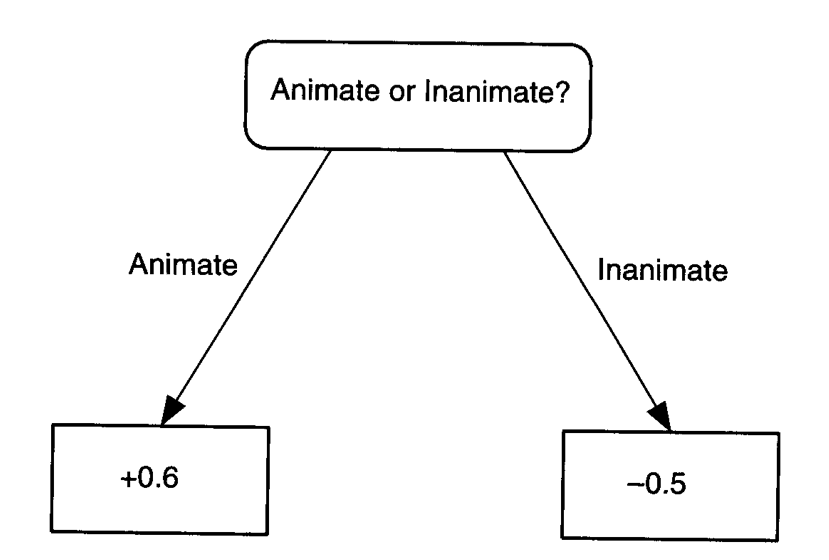
\includegraphics[width=100mm]{sources/images/TastyTree}\paragraph{}
    	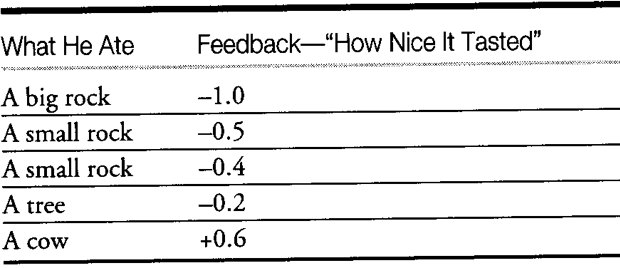
\includegraphics[width=100mm]{sources/images/TastyTable}
    	\caption{An example decision tree generated from the creature's experience eating objects \cite{:hc}.}
\end{figure}

After forming these trees from its previous experiences, a creature is able to form an opinion or prediction as to the outcome of performing a certain action. In the case of the simple example in Figure 4, the creature would deduce from experience that inanimate objects taste worse than animate ones, making it less likely to eat them in the future. 

In addition to learning from experience, the player also has the ability to reward or punish their creature when it performs certain tasks to further customise its learning. For example, if the player sees their creature eating a villager, they may choose to punish the creature to avoid the same thing happening in the future. This type of learning is accomplished using a type of reinforcement learning. 

In addition to this ``carrot and stick" method, the creature is also able to learn by watching the player's actions, and deducing what desire may have motivated the player to act in such a way. This dual approach stops the creature from falling into ``learning traps" by accidentally teaching the creature the `wrong' thing. For example, say the player wanted to teach their creature to avoid wolf creatures, but to be friendly to cow creatures. To do this, the player may punish the creature if they see it being friendly to a wolf creature. The creature may generalise from this punishment, and assume that it shouldn't be friendly to \emph{any} creatures, with no way for the player to correct the mistake. 

Where \emph{Black \& White}'s AI differs from other implementations of machine learning is that it utilises a combination of different methods to allow the agents to develop a unique personality, formed from its experiences of the world and the player. This combination of different techniques help the agents to avoid many of the pitfalls associated with machine learning techniques.

\section{Conclusion}

After researching different machine learning techniques and learning in games in general, I feel that reinforcement learning, and more specifically Q-learning is the most appropriate method for my problem area. One of the key reasons for this is that reinforcement learning methods excel at discovering optimal solutions to problems because of their use of the discount factor to take into account future rewards. This encourages the system to act optimally from the start. Another reason for choosing Q-learning being that it excels in situations where the system has no prior knowledge of its environment. Additionally, as my problem area is fairly limited, with a relatively small number of possible action/state combinations per level, I will be able to store the state/action/Q-value data in a table format; had I chosen a more complex problem with thousands of possible states, trying to store every combination would be impractical.

Of the other methods I researched, I feel that decision tree learning is another method which is suitable for my problem. However, I don't feel that using them for classification would fit my problem, as it would introduce unnecessary complexity; the obstacles that I'm using in my game are fairly basic, and trying to classify them would be unreasonable. Also, I don't feel that classification trees are suitable to the problem of learning an optimum route. Instead, I could use trees as a storage structure to dynamically map out the routes taken by an agent.

From my research, I have been made aware of a few issues which I will need to be aware of when designing my system. Firstly, I will need to make sure that my AI system doesn't learn the `wrong' thing, although this is unlikely as the system will not be influenced by the player at all. Another problem and one which may be difficult to work around is that of over-fitting (i.e. learning specific scenarios rather than generalised learning). However, as I am designing my system to learn to navigate specific levels, over-fitting is essentially the main aim. I may however be able to find a way to generalise the learnt knowledge so that it could be applied to other levels. 

Methods aside, what I found particularly interesting about my research was the systems which encorporate the learning into the game itself, allowing the player to customise how the game behaves. While this is not appropriate for all genres of game, I feel that this could add an extra level of customisability for the player, and perhaps help the player to bond with the AI agents in a way that just isn't possible with traditional static AI systems.

Another interesting point which was emphasised by my research was that intelligence truly is ``in the eye of the beholder" \cite{:hc}. An AI system's behaviour is judged differently according to the observer. What may consitute strong and entertaining AI to one person could be completely frustrating for another. While this could be a pitfall of utilising machine learning in games, I feel that if implemented correctly, it can mean that an AI system can be tailored to match different levels of players.
	
\chapter{Choice of Tools}

Although it may seem a fairly trivial task at first, choosing the right tools to develop my project was not an easy job; I had to make sure that the applications and engines/code libraries that I chose would be suitable for their intended purpose before I started any serious development, as trying to switch mid-way through the development process would undoubtably cause big problems were I to try and migrate the existing code to use other tools/libraries.

\section{Programming Languages \& Game Engines}

The first, and arguably the biggest decision I had to make was which language I was going to develop my project in. My choice of language would not only have a big influence on the performance (and so the scale of the game and the features I could develop), but also the hardware that my game would run on.  

I initially planned to develop my project in Java as I was already comfortable using the language, and liked its cross-platform nature. I decided to use the JMonkey engine for the game component, as it had powerful asset management, integrated GUI elements and applet integration to mention a few features. After carrying out a few simple tests however, I found it overly complex for my needs; it took a considerable abount of code to set up even a very basic scene. This isn't necessarily a fault of the engine itself, but rather of my choice to use 3D game engines in general; I had no need for the more advanced features such as complex physics and lighting etc. In addition, I didn't feel that 3D was particularly beneficial from an aesthetic point of view, considering my main inspiration was the classic 2D game Lemmings. I also had a few issues with a low framerate when adding many objects to the scene, which could cause me problems later on when I wanted to add many agents to the scene. Although this was likely due to my implementation rather than the engine itself, it highlighted to me the problems with developing in Java, and its lack of any memory management. Due to these points, I decided against trying to use a 3D engine and programming in Java.

My research eventually led me to Cocos2D: a 2D game engine originally written in Python, which has since been ported to many other languages including C++, Ruby and Objective-C. Using this engine opened up the possibility of developing my game for a mobile platform; something which greatly interests me (although admittedly, the JME does offer Android support).

I felt that Cocos2D was particularly well suited to my project as first and foremost, it is a well-established engine which is optimised for developing 2D games, with asset loaders, particle systems, and scene management to name a few of its useful features. It also comes bundled with two popular physics engines (Box2D and Chipmunk). Another point worth noting is that being a 2D engine, Cocos2D already has a thriving community of developers with experience making 2D games, whereas the JME is intended for 3D games, and as such, there was a lot less documentation for 2D games. 

Another benefit to using the Cocos2D engine is that it comes with libraries of code specifically optimised for games. For example, the engine comes with an alternative highly optimised collection class named `CCArray', which offers fast enumeration of its contents among other things. There is also a 'TextureCache' class which as the name suggests, caches textures in memory for quick access later. Cocos2D also offers sound support, integrated font rendering options, as well as some nice `automatic' (i.e. interpolatory) animation effects for moving objects smoothly on-screen. 

Although there is a port of the engine available for Java, I decided to develop my project in Objective-C for performance reasons that were outlined in my tests. Developing in Objective-C also meant that I could run my game on iOS devices. One of the main benefits to using Objective-C over Java is that it offers powerful memory management features, and so affords the developer much more control over their application. Although this may not be so much of an issue with modern desktop systems, the amount of available memory in a mobile environment is still fairly limited. Objective-C is also comparable to C++ in terms of runtime 'speed', due to the fact that Objective-C is essentially C (due to the fact that Objective-C is a strict subset of C) so any 'heavy lifting' code can be written in C if necessary to squeeze out the maximum performance. Objective-C also allows the developer to write code in C++ (called Objective-C++) if need be; something that would be necessary had I chosen to utilise the Box2D physics engine.

\begin{figure}[h!]
  \centering
    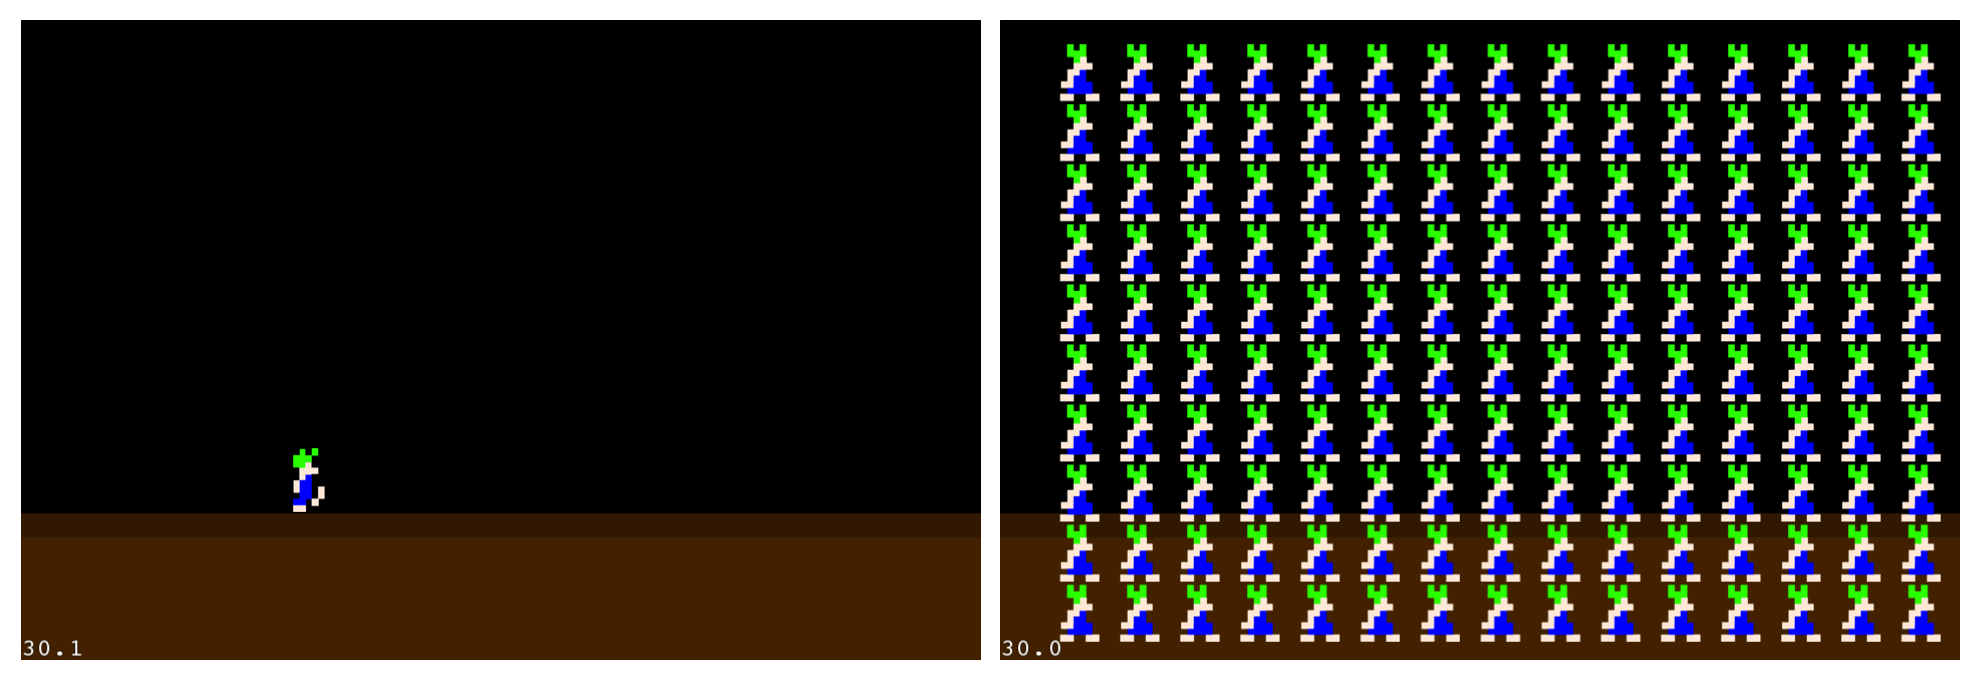
\includegraphics[width=140mm]{sources/images/InitialTests}
    \caption{Screens from my performance tests, both running at 30fps.}
\end{figure}

Before settling on the engine, I carried out a few basic performance tests to see if there were any performance bottlenecks similar to the issues I had with the JMonkey Engine. My first test was to add a single character to the scene, and animate it. My second test was to add more animating characters to see if there were any framerate issues; after adding 150 sprites, I was still achieving an impressive 30fps (see Figure 4 for screens). 

Another benefit to using Objective-C is having the option to use Apple's \emph{Xcode} as a development environment, as well as the bundled \emph{Instruments} performance profiling tools to get detailed analysis of the program's runtime performance.

\section{Asset Production}

Beyond writing the code for the game, I also needed to create a variety of assets for my game: backgrounds, character sprites, menu items, fonts etc. The Cocos2D engine supports a variety of image file formats, including the lossless PNG format which I would be using for the majority of my image assets. For the creation of my graphical assets, I used an image manipulation program called \emph{Pixelmator} which exports to PNG as well as a number of other formats. In addition to the raw image files, I also needed to create texture atlases (or sprite sheets) in order to take advantage of Cocos2D's optimised sprite batch node feature (discussed more in the implementation section). For the fonts, I used a program called \emph{bmGlyph}, which has been specifically developed for use with game engines that support the FNT file format.

\section{Version Control}

Using some form of version control system is a necessity in modern software development; it provides an easy way for multiple developers to collaborate on a single project (or even a single file) without causing file corruption. It is an invaluable tool for modern software development teams where it is not uncommon for developers to be in different cities or even continents. It also tracks all changes made throughout the development of the project. This is perhaps the most useful function of any version control systems as it not only allows the developers to see exactly what was changed (and by whom) in a project's history, but also means that were a mistake made, the project could easily reverted to an earlier state. Although I'm unlikely to experience any problems with file corruption as I'm the only one who will be contributing to the code-base, using a version control system still provides an incredibly useful way for me to not only track the progress of my project, but also as a way to incrementally back-up my project to ensure that any data loss is recoverable.

There are a variety of different source control systems available, such as CVS Subversion, Mercurial and Git. I decided to use Git as the version control system for my project for a couple of reasons. The first reason being that it is widely supported by many IDEs and other version control management software, with a number of services offering free Git hosting. I also generally prefer Distributed Version Control Systems (DVCS) as opposed to centralised systems for the reason that I like the freedom that DCVS systems give you in terms of being able to work on a project without the need for an internet connection. I also feel that DVCS systems provide more security in that each user has a backup of the entire system. However, this is not necessarily a benefit, as it could take up an inordinate amount of storage space were I working with many binary files (for example Adobe Flash files). In this case, using a DVCS would be unsuitable.

The Git version control system is actually very simple; it tracks all of the files in a project (known as the 'tree'), with each change submitted to the system (called a 'commit') consisting of a snapshot of the state of each file in the tree at that point in time. Specific commits can be 'tagged' to mark their significance; a feature which is normally used to mark specific releases of a project. Part of the reason Git is so efficient is that it uses an encoded string called a SHA hash (essentially a 'fingerprint' of the file) to determine whether or not a file has been changed; checking just requires comparing the local SHA to the remote SHA. 

I will be using a Git server hosted by GitHub to store the source code and documentation for my project. 

\section{Project Management}

To manage the progress of my project, I used a web-based application called ProjectPier which I installed on my web server so could be accessed from anywhere.

Using this system, I split my project into a number of 'task-lists' for each component in my project's development; for example: asset production, game development, AI development, testing, etc. I also added milestones to my project to mark specific targets that I wanted to achieve by certain dates.

Using this system, I could add individual tasks that needed to be completed, deadlines (or 'milestones') to mark specific targets in the development of my project. I could also use the system to create a wiki for my project containing useful information. 



%
% New part
%

\part{Planning}{This section covers the process of designing my system, from the initial concept art and art direction, to the system functionality modelling.}

\chapter{System Design}

\section{Design:} the designer must structure the programming tasks into a set of interrelated classes. Each class must be specified precisely, listing both its responsibilities and its relationship to other classes in the system.

\subsubsection{Main goals:}
\begin{itemize}
\item Identify the classes
\item Identify the responsibilities of these classes
\item Identify the relationships among these classes
\end{itemize}

Not necessarily a complete process; not all classes may be discovered until implementation.

\subsubsection{Components:} 
\begin{itemize}
\item A textual description of the classes and their most important responsibilities
\item Diagrams of the relationships among the classes
\item Diagrams of important usage scenarios
\item State diagrams of objects whose behaviour is highly state-dependant
\end{itemize}

\chapter{Artwork}
	
After designing a more concrete specification for my system, I created some initial artwork to establish how my game would look. In addition to the art style, I created some designs for how my levels would be composed with respect to how I intended to program my system in the implementation stage.
	
\section{Sprite Design}
	

	
\begin{figure}[h!]
  \centering
    
\includegraphics[width=80mm]{sources/images/Final}
    \caption{Final designs for agent sprites}
\end{figure}
	
\chapter{Social, Legal, Ethical and Professional Issues}
		\section{Intellectual Property}
		\section{Copyright Law}
		\section{The Data Protection Act}
		\section{Research Ethics}



%
% New part
%

\part{Implementation}{This section covers the process of actually implementing my system, problems that I was faced with, and how I solved them.}

\chapter{Coding Practices and Structure}

When writing the code for my project, I tried to stick to standard code formatting conventions and use standard design patterns where possible, as outlined in this section.

\subsection{Code Structure}

When setting up all of my files, I followed a common layout/structure as standard good programming practice, to ensure that my code was as easily readible to others as possible. I tried to keep the formatting the same in all places, and used a clear informative commenting style.

\subsubsection{Commenting}

I made sure that all of my source code files follow a certain comment format. The filename, project name, class description and the date the class was created at the very top of the file. Each method is then commented, with a brief description and any parameters/return variables specified. I tried to avoid commenting variables wherever possible, instead choosing to use variable names which are self-descriptive. See below for comment formatting.

\begin{lstlisting}
//
//  File name
//  Project name
//
//  Class description
//
//  DD/MM/YYYY: Created class
//

/**
 * Method description
 * @param any parameters
 * @return the returned objects
 */\end{lstlisting}

\subsubsection{Methods}

The format of my method headers is fairly standard, however, I prefix all method parameters with an underscore as it helps to clarify which variables in a method are parameters if quickly scanning the code.

\begin{lstlisting}
-(void)addLemming:(CCSprite*)_lemmingToAdd;
\end{lstlisting}


\subsection{Singleton Classes} 

I made a lot of use of the singleton design pattern throughout my project to create various 'manager' classes to deal with the shared data in my system. A singleton class is a special kind of class which only has one instance; calling a singleton instance will always return the one instance of the class, regardless of which class called it. The major benefit of using the singleton pattern being that you only need to store the data in one location, which can then be accessed by any class anywhere in the program (provided that the access to the data is restricted to a single thread at a time to avoid concurrency issues). My LemmingManager class which handles all of the agents in the game is an example of where I have used this pattern. It hold the only list of the characters in the game, and contains the functionality to add and remove lemmings among other things.

\subsection{Constants} 

I created a file to contain the read-only constant variables used in my program (for example the framerate, the default font filename and the various rewards associated with reinforcement learning). Moving all of these variables into a single separate file means that Each constant in this file follows the standard naming convention for constants (i.e. starting with a "k"). This is a legacy feature from the pre-Mac OS X days, possibly back when the Mac OS was written mostly in Pascal. 

\subsection{Datatypes} 

In addition to the constants file, I also created a similar file which contained many common datatypes which I would be using in my game. Types such as machine learning type, terrain type, character state, game rating and so on. As with the constants, this meant that I could keep all of the needed datatypes in a common location for easy access.

\subsection{Utility Methods} 

I created a Utils class with some useful static-access 'utility' methods which I was likely to want to use a lot in my game; functions such as random number generation, enumeration-to-string conversions, and timestamp generation. It made sense to create a separate class with all of these types of methods because it not only cut down on the amount of code that I had to write, but also meant that were I to find a bug in my random number generation code for example, I would only need to fix the bug in one place, rather than having to go and search every source file for occurrences of the broken code. 

\chapter{Game Component}
		
\section{Code Structure/Features}

Before I could build any learning into my project, I first had to create the underlying game component which would run it. As I was using the Cocos2D engine, a lot of the very low-level functionality had been taken care of. For example, the direct OpenGL ES calls needed for loading and binding textures were all contained within the CCSprite class. However, I still needed to take care of loading levels, adding objects, game characters, animating characters etc.

\subsection{Cocos2D} 

The Cocos2D framework comes with a very useful code library with various optimisations and utility methods which I made use of when implementing my game.

As previously mentioned, Cocos2D comes with a number of different base classes which can be used and take care of a lot of the very low-level OpenGL API calls. These classes have a heirarchical structure, using an analogy of film production to make this easy to understand. At the highest level is the CCDirector class which, as one would expect, controls the running of each individual level in the game (known as scenes). Scenes are essentially any new `screen' in the game, so are not necessarily just game levels, but can also me menu systems, game over screens and so on. Each scene consists of one or more layers which contain the actual game objects (for example background images, any level terrain and the game characters). The game objects (known as sprites) are at the bottom of the heirarchy and are just essentially an image with no real functionality by default.

The Cocos2D framework is loaded via the AppDelegate singleton class, which controls with the basic running of the iOS application; what should happen when launching the app, when the user closes the app, when the app is sent to the background etc.

In addition to the basic classes mentioned above, Cocos2D comes with a number of other useful features, such as the ability to add `transitions' in between scenes. The Cocos2D library also comes with a very useful CCAction class which allows the programmer to easily ass basic animations to sprite objects by simply specifying a start and end position and a duration. The class then creates an animation by interpolating between these two points. I use these actions in a number of places throughout my game, from animating the main menu items, switching graphs in the game stats screen, moving the agents in the game, and animating the game's pause menu. 

There are also some highly optimised data structures available, the most prominent being the CCArray class, which is a basic collection class which has been optimised for high-performance, with some methods that allow fast enumeration.

\subsection{Physics}

I initially intended to use one of the physics engines bundled with Cocos2D for the physics in my game. However, as the only physics required in my game was some basic collision detection and some way to simulate the agents `falling', I decided to write the required code myself to cut down on the processor time required. The other benefit to programming the physics and more specifically the collision detection myself is that I could customise which objects were included in the collision checks. This meant that I could optimise performance even further by ignoring any agent-to-agent collisions for example.

For the actual collision detection itself, I used basic bounding box detection as I had no need for anything more accurate. I made use of a method in the CCNode class (which my agents inherit from) which generates a bounding box for any given sprite. To detect whether any two objects were colliding, I made used of a utility method from the iOS code library \emph{CGRectIntersectsRect} which as the name suggests, checks if two rectangle objects intersect each other.

To simulate the agents `falling', I simply used a `CCAction' which basically creates an animation by interpolating between the start and end positions, similar to a `tween' in Adobe's ActionScript/Flash platform. 

\subsection{Levels} 

When it came to designing how the levels would work in my game, I wanted something which was very flexible, so that I could easily add extra levels (or modify existing ones) with a minimal amount of work. The way that I decided to do this was to create a number of generic assets which I could re-use in each level. Things such as platforms, water hazards, trapdoors etc. This meant that when I wanted to add an additional level to the game, I could simply specify the positioning of these existing elements, rather than having to create new level assets per level. By using re-usable assets, not only was adding new levels a lot simpler, it also meant that I could drastically cut down on the amount of disk-space that my game needed.

To accompany the assets, I also needed some way to specify the layout of each level, as well as other level specific data. To accomplish this, I used the natively supported Property List (plist) file format. Plist files are simply XML files of dictionary objects, consisting of a key object (usually a string), and a `value' object. One of the advantages to using the plist is that it's easily editable in any text editor. It also supports a variety of datatypes, such as strings, numbers (ints, floats, etc) and dates. Dictionaries can also be nested inside each other for even more flexibility. 

I use one plist file which specifies the levels in my game, along with certain level-specific information such as difficulty, number of tool uses etc. This file is loaded in, which tells the system how many levels need to be loaded, as well as their names. I then created a plist file for each level, which stored the positions of each piece of terrain, the type of terrain, and in some cases whether the terrain was collideable (this was enabled by default, so was only included if the object was to be removed from collision detection).

After loading in these plist files, I needed to translate the loaded data to into tangible game objects which could then be added to the game. To do this, I created terrain (i.e. platforms and floors) and obstacle (i.e. water, stampers etc.) classes which would encapsulate the required functionality. These classes contained the code necessary to create the sprites from the correct image files, and store the coordinates of the sprites according to the data loaded from the level's plist file. I also created a TerrainLayer class too keep all of the terrain objects separate from the other game objects. This class also deals with the actual loading of the plist files

Initially, I planned to have levels of varying difficulty, with an option on the new game screen to allow the user to select a difficulty. However, I found it difficult to determine what an 'easy' level should be for example, and so the final game just assumes all of the levels are the same difficulty. 

\subsection{Basic Agent Functionality}

Before I could program any of the machine learning into my agents, I first needed to set up some basic functionality such as animating and moving the agents and the ability to change state as well as some other basic behaviour.

I first programmed the animation for the characters, which involved splitting the animations into individual frames (see Figure 6) which could then be loaded into my game. To specify the frames needed for each animation, I created an external plist file which also listed the order of the frames, and the animation's length. 

\begin{figure}[h!]
  \centering
    
\includegraphics[width=60mm]{sources/images/Lemming_walk_anim}
    \caption{Frames Used for the Agent's Walking Animation}
\end{figure}

In addition to the animations, I also needed to set up some other basic behvaiour. I used a finite state machine which encapsulated all of the basic states for my agents: spawning, falling, idle, walking, floating, dead and win (i.e. reached the exit). Using this state machine, I could adjust the behaviour of the agents according to various in-game stimuli, and play any animations as appropriate. An example being when a falling agent collides with the ground, it transitions to the walking state. I also had to code a basic `fall timer', which counted how long an agent had fallen for, setting the next state to either walking, or dead if the fall was longer than a certain threshold. By this stage, I had set up my agents to spawn into the level at the correct point and move around the level from left to right, until they reach an immovable object at which point they turn around. I had added terrain objects and obstacles which changed the agent's state as appropriate (to `dead' if agent falls into water for example). The agents would respawn in killed, and the game would end if they successfully reached the level exit. At this point, my agents acted exactly as the characters in the original \emph{Lemmings} game, with no reasoning or other `intelligent' behaviour attached to them.

\subsection{Performance Optimisations} 

As already mentioned, Cocos2D offers a variety of performance optimisations specifically tailored for developing games. One such optimisation is the 'CCSpriteBatchNode'. It is not uncommon to experience poor performance when there are a large number of objects onscreen at once. 

For each sprite, OpenGL ES must first bind to the texture, and then render the sprite. As more and more sprites are added to the screen, it isn't difficult to see that the number of calls to OpenGL will steeply increase too, with every call costing a few CPU cycles. It is basic common sense to see that the game will run faster the fewer calls to OpenGL are made. 

The CCSpriteBatchNode is a Cocos2D class which has been created to help with this problem. The CCSpriteBatchNode works by taking a single texture which contains all of the textures needed by the current scene (called a texture atlas, see Figure 7), and sends all of the images for rendering to OpenGL at once, rather than individually. This essentially reduces the number of bind calls needed from O(n) to O(1) (in Big-O notation). Using texture atlases also cuts down on the amount of memory needed to store each individual image. In some version of the iOS, textures were required to be stored in sizes of the poet of two (64, 128, 512 etc.). This meant that the textures would often have a lot of unnecessary white space around the image, which obviously takes up extra memory; something which even with todays devices is not a commodity. An additional optimisation which can be made regarding the textures is to use the compressed PVR CCZ file format. In addition to saving disk space in terms of the actual size of the image, the PVR CCZ format is supported natively by the iPhone's GPU, and can be loaded directly onto the GPU without the need for conversion.

\begin{figure}[h!]
  \centering
    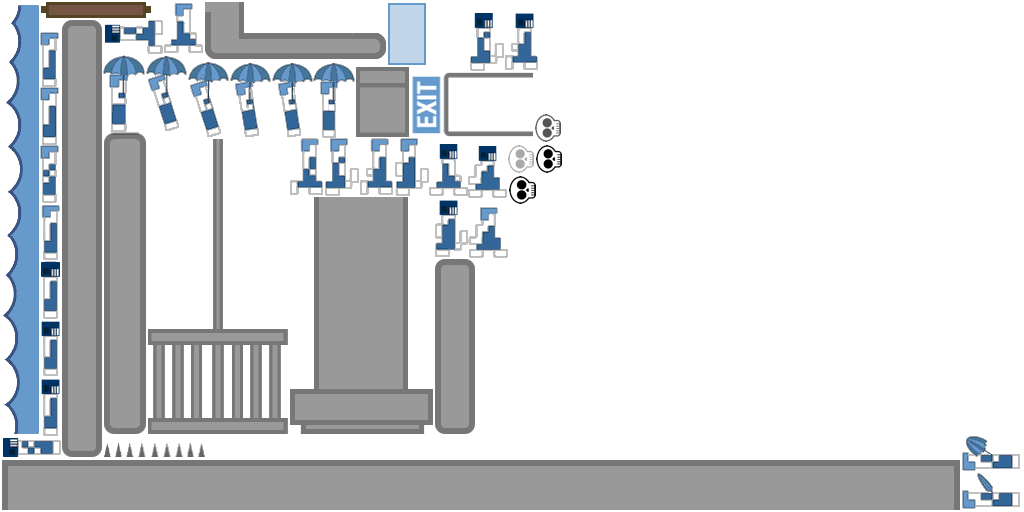
\includegraphics[width=100mm]{sources/images/Texture_atlas}
    \caption{An Example Texture Atlas}
\end{figure}

Aside from the performance optimisations offered by Cocos2D, I also did a few other things to ensure that my program ran as efficiently as possible.

\subsubsection{Random number generation} 

Although it may not seem like a likely source for a performance bottleneck, the random number generator (RNG) I chose to use could have a noticeable impact on performance. Based on some very quick tests carried out by a poster on the official Cocos2D forums \cite{:2011zt}, I was surprised to see the difference in speed between different RNG (see Figure 8). Typically, the RNG I had chosen to use (arc4Random) was by far the slowest method tested. Based on the tests carried out, I instead decided to use the CCRANDOM\_0\_1 function, which was shown to be 5 times quicker. Although the tests carried out on the forum were tested by performing 5 million iterations of the algorithm, far more than I would ever need to use, every performance enhancement helps.
	
	
\begin{figure}[h!]
  \centering	
	\begin{tabular}{|l|c|c|}
\hline
Algorithm & Device Time & Simulator Time \\ \hline
\multirow{5}{*}{Ranrot} & 0.037202 & 0.004751 \\
 & 0.036453 & 0.004786 \\
 & 0.037306 & 0.005023 \\
 & 0.036244 & 0.005536 \\ 
 & 0.037261 & 0.005243 \\ \hline
\multirow{5}{*}{UNI (multiply with carry)} & 0.287225 & 0.014551 \\
 & 0.286778 & 0.014798 \\
 & 0.285554 & 0.016061 \\
 & 0.286738 & 0.014633 \\
 & 0.288803 & 0.016177 \\ \hline
\multirow{5}{*}{CCRANDOM\_0\_1 (C random)} & 0.504273 &  \\
 & 0.498741 &  \\
 & 0.572036 &  \\
 & 0.498766 &  \\
 & 0.503112 &  \\ \hline
\multirow{5}{*}{xorrand} & 1.880982 & 0.093661 \\
 & 1.947728 & 0.101897 \\
 & 1.869296 & 0.090943 \\
 & 1.866257 & 0.091044 \\
 & 1.868058 & 0.096747 \\ \hline
\multirow{5}{*}{arc4random} & 2.970779 &  \\
 & 2.782961 &  \\
 & 2.973706 &  \\
 & 2.781113 &  \\
 & 2.785057 &  \\ \hline
\end{tabular}    \caption{Performance Tests of Random Number Generators}
\end{figure}
		
\section{Problems Faced} 

Something which I found particularly tricky about using Objective-C over a language like Java was the memory management. Learning Objective-C really emphasised to me how much the Java runtime shields the programmer from the low-level bugs associated with memory management thanks to its garbage collector. In Java, memory is reserved for an object simply by using the 'new' keyword, and memory is automatically released when that object goes out of scope and is no longer accessible. On the other hand, languages such as Objective-C  require manual memory management, meaning that every object created needs to be manually released by the programmer when finished. While the Objective-C language does come with a few optimisations which make memory management easier, it still caused me a number of problems. 

I found that the biggest problem with memory leaks is that they can often go undetected, only to cause the program to unexpectedly crash later on down the line. For this reason, they can be notoriously difficult to track down. I discovered a particularly nasty bug for example in my game's update method for example, which is called every frame, whereby I was allocating an array to hold all of the game objects, but failing to release the memory at the end of the method. This was a relatively small leak, but it was causing my game to drop 10+ frames per second if run for over 10 minutes.

I found another seemingly insignificant bug in my update method which was causing me to drop 15 frames per second after the game had been running for about 15 minutes. The bug was caused by a careless error I made when initialising the game. When the game was first initialised, I wanted to create a list of all collideable objects, for use in collision detection later. To do this, I put code in the update loop which added every object to a list. However, rather than just adding the objects once when the game was initialised, I found that I was re-adding each object every frame, causing a huge issue with performance. After just 10 seconds, I found that my list of collideable objects contained over 10,000 objects, which was obviously causing big problems when it came to my game trying to check for collisions.

Luckily, Xcode comes with a very useful set of performance analysis tools called 'Instruments' which can be used to establish any memory-related or runtime issues, such as memory leaks etc. Instruments allows you to test your app in `profiling' mode, which tracks what memory has been allocated, and suggests areas where memory leaks may occur.

Carrying out this project really taught me the importance of keeping a close eye on what memory I was allocating and where it was being released. What may at first seem like a negligible memory leak can build up over time, and combined with other similarly small memory leaks, can cause big problems with your programs performance. I would even go so far as to say that these smaller memory leaks are even more troublesome than the bigger ones, as they are much harder to track down, and are often more widely spread, and therefore more difficult to fix.

Another problem I frequently came across which couldn't happen in memory-managed languages like Java was that of uninitialised variables. Whereas in Java, whenever you declare a new variable, it's automatically initialised with whatever the default value may be, you get no such privilege in Objective-C. When you declare a variable in Objective-C, it stays uninitialised until you specifically set it. This caused me the biggest problems with arrays; trying to access an uninitialised array wouldn't cause a compiler error, but would cause an unexpected crash at runtime.

\chapter{AI Component}

After the core game component had been implemented, I could start to build the AI learning system. My first task was to update the levels 

\section{Level Structure}

In order to simplify the decision making process, I split my levels into a number of `nodes' (See Figure 9). These nodes represent decision points in my levels; areas where there are more than one possible path forward, where the agent has to decide which route to take. As trapdoors had already been placed in the level, these were used as one type of decision node. I also needed to create an additional invisible decision object which could be at the end of platforms or anywhere where I couldn't place a trapdoor. 

\begin{figure}[h!]
  \centering
    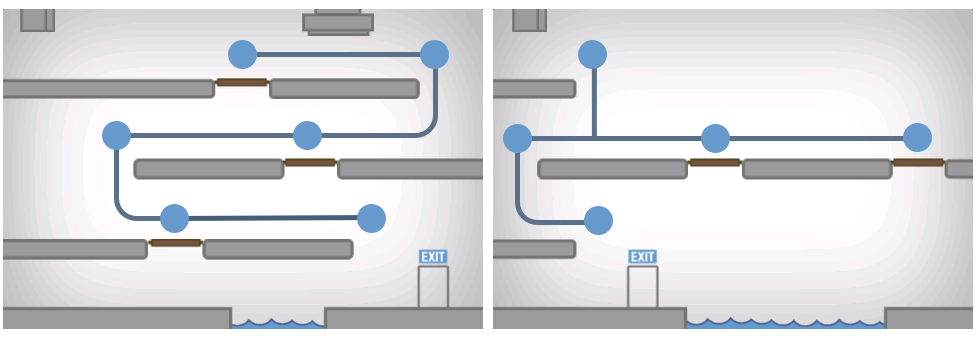
\includegraphics[width=140mm]{sources/images/LevelNodes}
    \caption{Decision Node Graphs for Two Levels}
\end{figure}

\section{Learning Agents}

In my final game, I implemented three alternative methods of learning: a shortest route method, a modified decision tree method, and a reinforcement learning method using the Q-learning algorithm. I explain the different implementations used in my game in this section.

As I intended to implement more than one learning technique, I designed the code for my game characters in such a way that the AI was completely self-contained in its own class. Not only is this generally good object-oriented design, but it also meant that to use a different type of learning, all I had to do was to link the relevant class, no other changes were required. This functionality could be neatly implemented in a switch statement (See figure 9)

\begin{figure}[h!]
\begin{lstlisting}
switch(learningType) 
{                
	case kLearningMixed:
    	// randomly choose a learning type
        learningType = [Utils generateRandomNumberFrom:0 to:kLearningMixed]; 
        break;
                
    case kLearningReinforcement:
        class = [QLearningAgent class];
        break;
                
    case kLearningTree:
        class = [DecisionTreeAgent class];
        break;
                
    case kLearningShortestRoute:
        class = [ShortestRouteAgent class];
        break;
         
    case kLearningNone:
        class = [CogitoAgent class];
        break;
                
    default:
        break;
}
\end{lstlisting}
\caption{Switch Statement for Setting Learning Type}
\end{figure}

As outlined in my initial design, the learning agents begin the game in a `learning mode', in which they have a set number of lives or `episodes'; the number of learning episodes is set by the player before the game begins. During learning mode, the agents navigate the level and choose actions at random, building up their knowledgebase. 

I initially planned to set up the learning such that after the first episode, the agent would cease to act randomly and apply its knowledge. However, I found that doing this made it extremely difficult to measure the improvement in the characters, as once they reached the exit, the game was over. Instead, I decided to implement the learning mode which avoids this issue. Additionally, by programming the agents to act randomly throughout the learning mode meant that more optimal routes were found in less time, due to the fact that there was no `exploitation' of current knowledge at this stage. In many reinforcement learning systems, the system begins to exploit the learnt knowledge much earlier on, which brings with it the added issue of balancing the exloitation of existing knowledge with the exploration of new terrain. 

After all of the learning episodes have been completed, learning mode ends the agent then applies the knowledge it has learnt to attempt to reach the exit safely.

\subsection{Cogito Agents}

I created a base class called \emph{CogitoAgent} to contain the common functionality which would be shared between all types of learning. Its most basic function is to detect when an agent has reached a decision node, at which point it chooses a random action from those avalable. The class also keeps track of the number of learning episodes used by the agent, and ends the learning mode when all episodes have been completed.

\subsection{Shortest Route Agents}

The Shortest Route agent is the simplest and most naive of all of the learning types. Shortest Route agents record the routes which have been taken during the learning mode. I created a Route class to simplify this, which itself consists of an array of `nodes' and a boolean flag which stores whether or not the route was successful (i.e. if the agent survived or not). Upon completion of the learning mode, the Shortest Route agent checks all of the routes taken, chooses the shortest one, and takes it. If there happens to be several shortest routes of the same length, the agent doesn't attempt to compare the routes, but just picks the first one it finds. If the agent failed to reach the exit during the learning mode, it simply acts randomly.

\subsection{Decision Tree Agents}

As shown in my research, decision tree learning is usually used for classification problems, whereby an agent finds itself in a certain situation, and it uses a decision tree to try to `classify' the situation using knowledge it has gained from experience. Initially, I planned to use this approach in my game. However, I felt that it was an overly complex solution to what is a relatively simple game concept. I didn't think that there was any point in trying to create diverse obstacles which required the agent to have to classify them; it just seemed unrealistic. I felt that trying to use classification techniques to solve my problem of terrain navigation was inappropriate
 
Instead, I decided to use tree structures to allow my Decision Tree agents to function in a similar way to the Shortest Route Agents. Like the Shortest Route agents, the Decision Tree agents record the routes taken, with the shortest routes being chosen after the learning mode is complete. However, there are some subtle changes which make this method more accurate than the Shortest Route method. The obvious difference is that the routes are stored in a tree structure, which is built dynamically as the agent experiences the world. 

To implement the tree structure, I created a \emph{TreeState} class. The class stores references to the parent and child nodes, and has code to add child nodes to the tree. There is also a boolean flag which stores whether the particular TreeState is a leaf node.

When searching for the optimum route, the routes are all given `weightings'. The weighting for a route is based on the number of tools used in that route; a route with no tool uses has a weighting of 0, with the weighting being incremented by 1 for every tool used. 

\subsection{Reinforcement Agents}

The reinforcement agents are the most complex agents in my system.

Asynchronous approach of updating the Q-values; updating a single pair at the end of every episode (synchronous - update all episodes once)

\section{Other Features}

In addition to the agent classes, I also implemented a few other useful AI-related features into my game.

\subsection{Learning Knowledgebase}

\subsection{Learning Stats}

\section{Problems Faced}
	
	
	
%
% New part
%

\part{Testing \& Evaluation}{This section presents the usability and learning testing I performed, the results that were obtained, and an analysis of the product's performance.}

\chapter{Testing \& Results}

Show the results of usability testing (if any) and the learning results. Compare with the different types and no learning, show graphs to compare. Discuss the effectiveness, advantages/disadvantages to the learning algorithms used.

\section{Usability Testing}

Pause bug

\section{AI Testing}



%
% New part
%

\chapter{Evaluation}

A very competent evaluation of the whole project (with hindsight). Weak performance in the evaluation of product and process will result in a grade no higher than a B.

\section{Time Management}

Initial plan was to use a waterfall development approach (discuss). Eventually took a slightly more incremental approach: developed game and AI together towards the end, some asset creation throughout. Discuss why, which would have been better - for one person rather than a team. As I was unfamiliar with the language and the engine, it was difficult to decide how best to approach the design/implementation. (see \url{http://en.wikipedia.org/wiki/Software_development_methodology})
		
- Waterfall: a linear framework
- Incremental: a combined linear-iterative framework
- Spiral: a combined linear-iterative framework
		
The biggest miscalculation with regards to my time-management and project schedule was that I failed to recognise just how much groundwork was needed to build the game component. Though I by no means expected the game development to be a trivial task, I wasn't prepared for the amount of work that was needed. This was exacerbated by the fact that I was also still getting to grips with Objective-C, and so my productivity wasn't as it could have been. However, although I slipped by a couple of weeks during the game development stage, I finished the AI component of the game under-schedule. Looking back at the volume of code that was needed to get the game running, it seems fairly that I should have at least allocated an equal amount of time to both the game and AI components. As it happens, I still finished my project to schedule with some time to spare.

\section{Game Evaluation}

\section{Machine Learning Evaluation}

- space required for storage
- pros
- cons
- possible improvements

\subsection{Analysis of Shortest Route Learning}

Shared knowledgebase

very naive, needs some way to compare different routes. If no route is found, the agent acts randomly. The larger the levels, the less likely it is that the agent will reach the exit alive.

Quick to function - no need to traverse trees etc.

\subsection{Analysis of Decision Tree Learning}

Shared knowledgebase

Slower than Shortest Route
Would like to implement more powerful route filtering; perhaps add the weighing onto the route length? Maybe implement A* search in anticipation of much larger levels.

\subsection{Analysis of Reinforcement Learning}

A big benefit to reinforcement learning is that every decision made, whether good or bad, contributes to the knowledgebase in a positive way; if an agent dies, that episode is still as helpful as if the agent had reached the exit (if not more, as it teaches the agent where \emph{not} to go)

\subsection{}

My problem area is very limited

+ it can handle uncertain and noisy domains
+ it can interface with an external world more easily than other methods
- slow learning rate as they rely on backwards propagation of rewards. The problem solver must pass through early parts of the problem space many times before any rewards at all reach those locales.

1. Large state/action space. Since games usually have several different types of objects and characters and many different possible actions, the state/action space that RL must explore is extremely high dimensional. Dealing with high-dimensional spaces is a known challenge with RL in general (Sutton and Barto 1998), but in a real-time game there is the additional challenge of having to check the value of every possible action on every game tick for every agent in the game. Because traditional RL checks all such action values, the value estimator must execute several times (i.e. once for every possible action) for each agent in the game on every game tick. Action selection may thus incur a very large cost on the game engine, reducing the amount of computation available for the game itself.

2. Diverse behaviors. Agents learning simultaneously in a simulated world should not all converge to the same behavior: A homogeneous population would make the game boring. Yet because many agents in video games have similar physical characteristics and are evaluated in a similar context, traditional RL techniques, many of which have convergence guarantees (Kaelbling et al. 1996), risk converging to largely homogeneous solution behaviors. Without explicitly maintaining diversity, such an outcome is likely.

3. Consistent individual behaviors. RL depends on occasionally taking a random action in order to explore new behaviors. While this strategy works well in offline learning, players do not want to constantly see the same individual agent periodically making inexplicable and idiosyncratic moves relative to its usual policy.

4. Fast adaptation and sophisticated behaviors. Because players do not want to wait hours for agents to adapt, it may be necessary to use a simple representation that can be learned quickly. However, a simple representation would limit the ability to learn sophisticated behaviors. Thus there is a trade-off between learning simple behaviors quickly and learning sophisticated behaviors more slowly, neither of which is desirable.

5. Memory of past states. If agents remember past events, they can react more convincingly to the present situation. However, such memory requires keeping track of more than the current state, ruling out traditional Markovian methods. While methods for partially observable Markov processes exist, significant challenges remain in scaling them up to real-world tasks (Gomez 2003).

There is no danger of my agents learning the `wrong' thing due to the fact that they learn entirely from their own experiences and take no input from the player.

\section{Areas For Enhancement}

Although I'm very pleased with the outcome of my project, given extra development time, there are a number of areas which I feel I would like to extend further.

The most obvious enhancement that I could make would be to extend the AI system to incorporate more learning types. Were I to do this, the next learning algorithm that I would like to try would be a genetic algorithm, as I think that it lends itself quite well to the context of my game. I could slightly alter the spawning of the lemmings so that they all spawn in waves, a certain number at a time - say 100. Then, at the end each wave, I could evaluate each lemming's performance, choosing to breed those with the most effective policy.

Another enhancement that I think it would be interesting to make would be to allow for multiple learning types to be used in a single game, with separate agents able to use different algorithms. It would be interesting to compare the performance of the two. Following on from this idea, I also think it could be interesting to mix different methods of learning together in one lemming…

Something else which I'd like to implement would be some way for the agents to learn from each other - perhaps by watching other agents. This obviously wouldn't work with the shared knowledge base, but would be interesting to see the improvement of learning this way over the original.

Another enhancement that I could make to the game would be to extend the system to a 3D environment. This would obviously complicate things, but.

\begin{itemize}
	\item Implement additional learning types
	\begin{itemize}
		\item Mixed learning types between agents
    	\item Use a combination of types
    \end{itemize}
    \item Remove the random learning episodes
    \item Communication between agents (shared knowledge base?)
    \item Extend to a 3D environment
    \item Level editor
    \item Bigger levels (multiple screens) - Although there's a definite improvement, I don't feel that the small levels allow my system to really show off what it can do. I would like to have maybe created levels which spanned multiple screens, although I made the decision not to do this for usability reasons (there'll always be some part of the screen which is obscured). 
    \item Overfitting - design a more general system
    \item "Start with a large correction factor (learning rate), and slowly decrease the parameter, which gives the algorithm a rough approximation during the early stages and allows fine tuning later in learning."
    \item Test alternative reinforcement methods (bucket brigade, temporal difference) 
\end{itemize}

Negatives of using reinforcement learning: it doesn't generalise beyond specific states (over-fitting). Possible fix: use genetic algorithms - "the expected reward on production rules serves as their fitness, with more fit rules being selected for reproduction. The new rules are then evaluated by running them in an environment, with the best of them being selected to produce another generation, and so on. Such classifier systems are often used in conjunction with the bucket brigade algorithm for determining expected rewards."

\section{Conclusion}

I feel that the possibility of utilising academic machine learning techniques into commercial computer games is an often overlooked technique which is not only possible, but feasible with todays technology; something I have proven by showing this on a mobile platform. 

- Applications For Learning in games (possibly pre-release learning)
- Performance on mobile device

Taught me important lessons about game design - things which may not be so necessary today with the powerful hardware as standard (with even mobile devices now sporting dual-core chips)

Machine learning in games could have many possible applications. The obvious use is to create much 'smarter' AI-controlled characters which are capable of modifying their behaviour dynamically to adapt to unforeseen scenarios. This could be applied to virtually any game genre, from enemy commanders in a real-time strategy war game, to the AI-controlled players in a football game, to more intelligent enemy characters in a platform game. Some applications are often more pertinent than others; performance is still of paramount importance, and is still an issues; mostly so with console games where the hardware capabilities is strictly limited, and even more so on mobile devices.

%
% New part 
%

\part{Appendices}{}

	\appendix
	
	\chapter{Code Listings}

	\chapter{Project Log}
	
A day-by-day work diary kept by you as the project is carried out. A log which has evidently been manufactured to be handed in rather than having been properly kept will result in a lower grade.

	\chapter{Git Log}


	
%
% References
%

\singlespace

\newpage
\addcontentsline{toc}{part}{Bibliography}
\bibliographystyle{abbrv}
\bibliography{Cogito}

\end{document}
